\documentclass[10pt,fleqn,a4paper]{jsarticle}
\usepackage[dvipdfmx]{graphicx,color}
\usepackage{ascmac,amsmath,amssymb,amstext}
\usepackage{tikz,multicol,float,tikz-3dplot}
\usetikzlibrary{positioning,intersections,calc,arrows.meta,math,angles,patterns}
\usepackage{zogeny,ceo,comment}
\newcommand{\theme}[1]{【\text{#1}】}
\newcommand{\ans}[1]{\mbox{\boldmath{$#1$}}}
\renewcommand{\baselinestretch}{1.3} 
\newcommand{\hokusomu}[1]{
\begin{tikzpicture}[scale=1]
\filldraw[fill=black,draw=black](0,0)--({1-0.2},{0})--({1-0.2},{1-0.2})--(0,{1-0.2})--(0,0);
\draw[-,thick](0,0)--({1-0.2},{0})--({1/2-0.2},{1-0.2})--(0,{1-0.2})--(0,0);
\node[white,font=\Huge]at({1/2-0.1},{1/2-0.1})(label){$\mathbf{#1}$};
\end{tikzpicture}}
\newcommand{\hokukai}{
    \begin{tikzpicture}
  \draw[line width=0.2mm](-0.73,{-1/4+0.04})--(-0.73,{1/4-0.03})--(0.73,{1/4-0.03})--(0.73,{-1/4+0.04})--cycle;
  \draw[line width=0.6mm](-0.73,{-1/4+0.03})--(-0.73,{1/4-0.02});
  \draw[line width=0.6mm](0.73,{-1/4+0.03})--(0.73,{1/4-0.02});
  \node at(0,0){\kurosankakub \ans{解答}\kurosankakua};
\end{tikzpicture}
} %全国大学入試問題の「解答」記号
\tdplotsetmaincoords{70}{115}%{xy平面からどれだけ上にいるか(90度から-90度)}{z軸中心にどれだけ左右に回転するか}
\title{数学の核心-別冊解答-Vol.2}
\author{大島　遙斗}
\begin{document}
\maketitle
\newpage
\tableofcontents
\newpage
\section{講義問題解答}
\newpage
\subsection{1章：ベクトルの移動・一次独立・斜交座標}
\noindent\ba{1$\bullet$1}\theme{単位ベクトル}\\
\kakkoichib$\vec{a}$と同じ向きに10進むベクトルは,$\dfrac{10}{|\vec{a}|}\vec{a}$なので,
\begin{align*}
  \Vec{OP}=\Vec{OA}+\dfrac{10}{|\vec{a}|}\vec{a}=\tvec<0,1>[-1,-1]+2\sqrt{5}\tvec<0,1>[2,1]
\end{align*}
$\Y \ans{\mathrm{P}\p{-1+4\sqrt{5}},1+2\sqrt{5}}$\\
\kakkonib$\Vec{AB}$の向きに18進むベクトルは,$\dfrac{18}{|\Vec{AB}|}\Vec{AB}$なので,
\begin{align*}
  \Vec{OP}=\Vec{OA}+\dfrac{18}{\Vec{AB}}\Vec{AB}=\Tvec<0,1>[1,0,-1]+\dfrac{18}{\sqrt{6}}\Tvec<0,1>[1,1,2]
  =\Tvec<0,1>[1,0,-1]+3\sqrt{6}\Tvec<0,1>[1,1,2]
\end{align*}
$\Y\ans{\p{1+3\sqrt{6},3\sqrt{6},-1+6\sqrt{6}}}$\\\\
\ba{1$\bullet$2}\theme{東北大-斜交座標系}\\
\kangaekata 斜交座標を使ってそれぞれの座標を出すことを考えましょう.\\
\hokukai\kakkoichib Aを原点とし,$\Vec{AB},\Vec{AC}$を基底とする$XY$座標系で考える.下図のようになる.
\begin{center}
 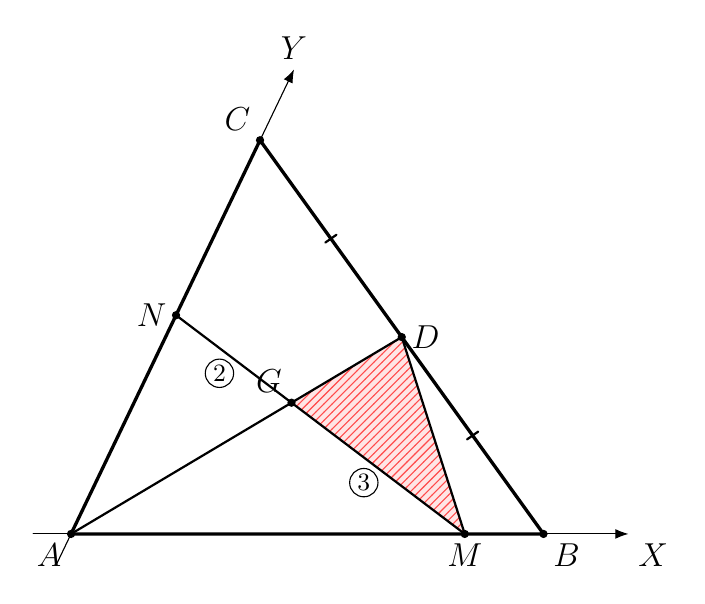
\begin{tikzpicture}[
  x={(6cm,0cm)},
  y={(2.4cm,5cm)},
  line cap=round,
  line join=round,
  every node/.style={font=\large}
 ]
  % 各点の斜交座標
  \coordinate (A) at (0,0);
  \coordinate (B) at (1,0);
  \coordinate (C) at (0,1);
  \coordinate (D) at (1/2,1/2); % CBの中点
  \coordinate (G) at (1/3,1/3);
  \coordinate (M) at (5/6,0);
  \coordinate (N) at (0,5/9);

  % 斜交座標軸
  \draw[->,>=Latex] (-0.08,0)--(1.18,0)
    node[below right,black] {$X$};
  \draw[->,>=Latex] (0,-0.08)--(0,1.18)
    node[above,black] {$Y$};

  % 三角形GDMの斜線
  \fill[red!10] (G)--(D)--(M)--cycle;
  \fill[pattern=north east lines,pattern color=red!70]
    (G)--(D)--(M)--cycle;

  % 三角形ABCと内部の線分
  \draw[very thick] (A)--(B)--(C)--cycle;
  \draw[thick] (A)--(D);
  \draw[thick] (N)--(M);
  \draw[thick] (D)--(M);

  % DがCBの中点であることを表す印
  \draw[thick] ($(C)!0.5!(D)$) ++(-2pt,-1.4pt)--++(4pt,2.8pt);
  \draw[thick] ($(D)!0.5!(B)$) ++(-2pt,-1.4pt)--++(4pt,2.8pt);

  % 点と点名
  \foreach \P in {A,B,C,D,G,M,N}
    \fill (\P) circle[radius=1.5pt];

  \node[below left]  at (A) {$A$};
  \node[below right] at (B) {$B$};
  \node[above left]  at (C) {$C$};
  \node[right]       at (D) {$D$};
  \node[above left]  at (G) {$G$};
  \node[below]       at (M) {$M$};
  \node[left]        at (N) {$N$};
  \node[draw,circle,inner sep=1pt,font=\small,below left=2pt]
  at ($(N)!0.5!(G)$) {$2$};
\node[draw,circle,inner sep=1pt,font=\small,below left=2pt]
  at ($(G)!0.5!(M)$) {$3$};
\end{tikzpicture}
\end{center}

これより,G$\p{\frac{1}{3},\frac{1}{3}}$,M$\p{\frac{5}{6},0}$,N$\p{0,\frac{5}{9}}$なので,
\begin{align*}
  &\mathrm{AM}:\mathrm{MB}=\dfrac{5}{6}:\dfrac{1}{6}=\ans{5:1}\\
  &\mathrm{AN}:\mathrm{NC}=\dfrac{5}{9}:\dfrac{4}{9}=\ans{5:4}
\end{align*}
\kakkonib 直線MDの式を求める.このとき,直交座標系で考えても比は変わらないので,下図を得る.
\begin{center}
  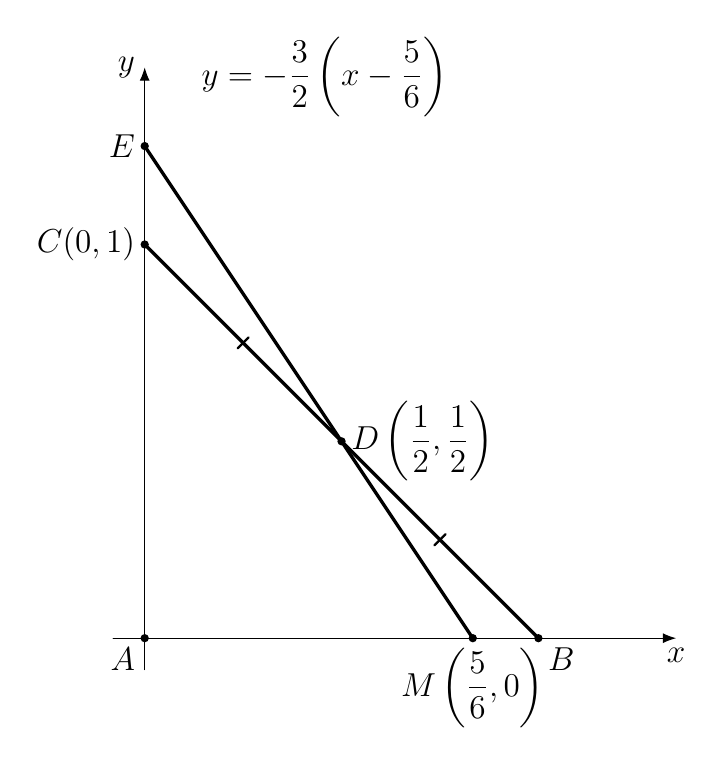
\begin{tikzpicture}[
  x=5cm,
  y=5cm,
  line cap=round,
  line join=round,
  every node/.style={font=\large}][]
  % 各点
  \coordinate (A) at (0,0);
  \coordinate (B) at (1,0);
  \coordinate (C) at (0,1);
  \coordinate (D) at (1/2,1/2);
  \coordinate (M) at (5/6,0);
  \coordinate (E) at (0,5/4);

  % 座標軸
  \draw[->,>=Latex] (-0.08,0)--(1.35,0) node[below] {$x$};
  \draw[->,>=Latex] (0,-0.08)--(0,1.45) node[left] {$y$};

  % 直線CBと直線EM
  \draw[very thick] (C)--(B);
  \draw[very thick] (E)--(M);

  % DがCBの中点であることを示す印
  \draw[thick]
    ($(C)!0.5!(D)$)++(-2pt,-2pt)--++(4pt,4pt);
  \draw[thick]
    ($(D)!0.5!(B)$)++(-2pt,-2pt)--++(4pt,4pt);

  % 点
  \foreach \P in {A,B,C,D,M,E}
    \fill (\P) circle[radius=1.5pt];

  % 点名・座標
  \node[below left]  at (A) {$A$};
  \node[below right] at (B) {$B$};
  \node[left]        at (C) {$C(0,1)$};
  \node[right]       at (D) {$D\left(\dfrac12,\dfrac12\right)$};
  \node[below]       at (M) {$M\left(\dfrac56,0\right)$};
  \node[left]        at (E) {$E$};

  % 直線EMの方程式
  \node[above right] at (0.12,1.30)
    {$y=-\dfrac32\left(x-\dfrac56\right)$};
  \end{tikzpicture}
\end{center}
これより,直線MDの式は,
\begin{align*}
  Y=-\dfrac{3}{2}\p{X-\dfrac{5}{6}}
\end{align*}
なので,これの$y$切片は,$\dfrac{5}{4}$より,E$\p{0,\dfrac{5}{4}}$\\
$\Y$AC:CE$=1:\dfrac{1}{4}=\ans{4:1}$\\
\kakkosanb 面積比はどの座標系で考えても同じなので,下図の直交座標系で考える.
\begin{center}
  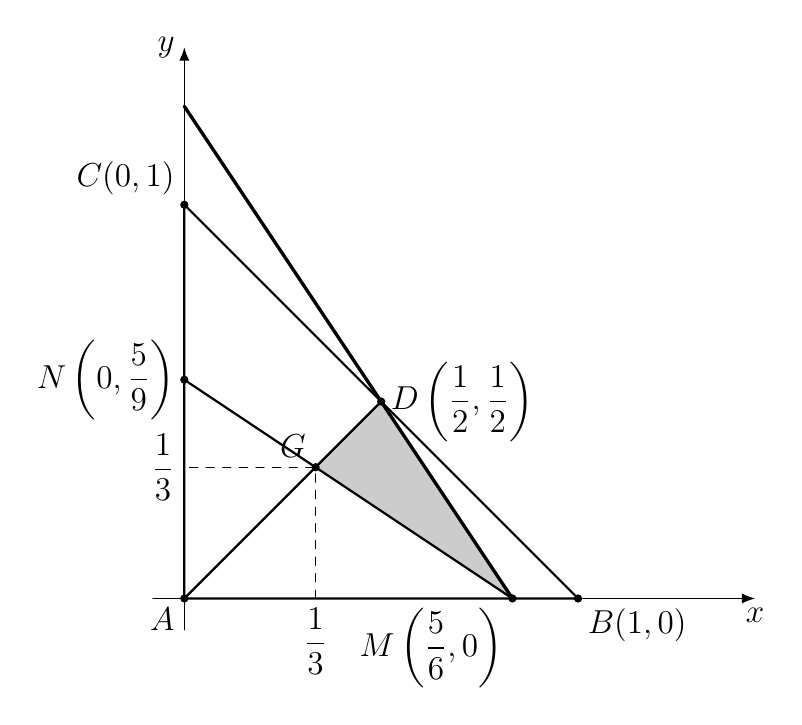
\begin{tikzpicture}[
  x=5cm,
  y=5cm,
  line cap=round,
  line join=round,
  every node/.style={font=\large}
]
  % 各点
  \coordinate (A) at (0,0);
  \coordinate (B) at (1,0);
  \coordinate (C) at (0,1);
  \coordinate (D) at (1/2,1/2);
  \coordinate (G) at (1/3,1/3);
  \coordinate (M) at (5/6,0);
  \coordinate (N) at (0,5/9);
  \coordinate (E) at (0,5/4);

  % 座標軸
  \draw[-{Latex}] (-0.08,0)--(1.45,0)
    node[below] {$x$};
  \draw[-{Latex}] (0,-0.08)--(0,1.40)
    node[left] {$y$};

  % 三角形GDM
  \fill[black!20] (G)--(D)--(M)--cycle;

  % 三角形ABC
  \draw[thick] (A)--(B)--(C)--cycle;

  % 内部の線分
  \draw[thick] (A)--(D);
  \draw[thick] (N)--(M);
  \draw[very thick] (E)--(M);

  % Gから座標軸への補助線
  \draw[dashed] (1/3,0)--(G)--(0,1/3);

  % 点
  \foreach \P in {A,B,C,D,G,M,N}
    \fill (\P) circle[radius=1.5pt];

  % 点名・座標
  \node[below left]  at (A) {$A$};
  \node[below right] at (B) {$B(1,0)$};
  \node[above left]  at (C) {$C(0,1)$};
  \node[right]       at (D)
    {$D\left(\dfrac12,\dfrac12\right)$};
  \node[above left]  at (G) {$G$};
  \node[below left]  at (M)
    {$M\left(\dfrac56,0\right)$};
  \node[left]        at (N)
    {$N\left(0,\dfrac59\right)$};

  % 1/3の目盛り
  \node[below] at (1/3,0) {$\dfrac13$};
  \node[left]  at (0,1/3) {$\dfrac13$};
\end{tikzpicture}
\end{center}
これより,
\begin{align*}
  &\Sankaku{ABC}=\dfrac{1}{2}\\
  &\Sankaku{DGM}=\Sankaku{ADM}-\Sankaku{AGM}=\dfrac{1}{2}\times\dfrac{5}{6}\times\dfrac{1}{2}-\dfrac{1}{2}\times\dfrac{1}{3}\times\dfrac{5}{6}=\dfrac{1}{2}\times\dfrac{5}{36}
\end{align*}
$\Y\Sankaku{DGM}=\dfrac{5}{36}\Sankaku{ABC}$\\
$\Y\ans{\dfrac{5}{36}倍}$\\\\
\ba{1$\bullet$3}\theme{斜交座標系による存在領域の図示}\\
$\Vec{OP}=s\Vec{OA}+t\Vec{OB}$,\hspace{5mm}$s,t$が$\begin{cases}
  s\geq0\\
  1\leq s+2t\leq2\\
  3s+t\leq3
\end{cases}$を満たす.これを,$\Vec{OA},\Vec{OB}$を基底とする斜交座標系で考えると,下図を得る.
\begin{center}
  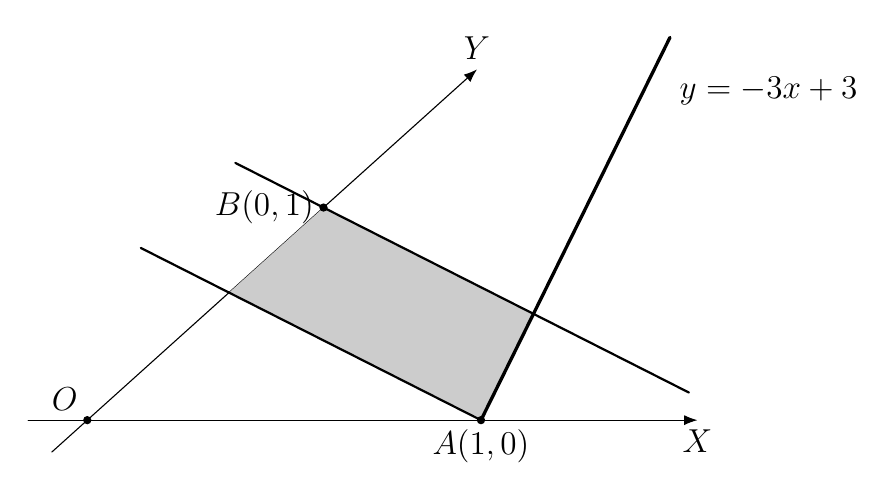
\begin{tikzpicture}[
  x={(5cm,0cm)},
  y={(3cm,2.7cm)},
  line cap=round,
  line join=round,
  every node/.style={font=\large}
]
  % 主な点
  \coordinate (O) at (0,0);
  \coordinate (A) at (1,0);
  \coordinate (B) at (0,1);

  % 斜線領域の残りの頂点
  \coordinate (P) at (0,3/5);
  \coordinate (Q) at (5/6,1/2);

  % 斜交座標軸
  \draw[-{Latex}] (-0.15,0)--(1.55,0)
    node[below] {$X$};
  \draw[-{Latex}] (0,-0.15)--(0,1.65)
    node[above] {$Y$};

  % 斜線領域
  \fill[black!20] (P)--(B)--(Q)--(A)--cycle;

  % 平行な2直線
  \draw[thick,domain=-0.35:1.45,samples=2]
    plot (\x,{-0.6*\x+1});
  \draw[thick,domain=-0.35:1.0,samples=2]
    plot (\x,{-0.6*\x+0.6});

  % 直線 y=-3x+3
  \draw[very thick,domain=0.4:1,samples=2]
    plot (\x,{-3*\x+3});



  % 点
  \foreach \X in {O,A,B}
    \fill (\X) circle[radius=1.5pt];

  % 点名
  \node[above left] at (O) {$O$};
  \node[below]      at (A) {$A(1,0)$};
  \node[left] at (B) {$B(0,1)$};

  % 直線の式
  \node[right] at (0.55,1.55)
    {$y=-3x+3$};
\end{tikzpicture}
\end{center}
比はどの座標系で考えても変わらないので,$xy$直交座標系で考えると,次図を得る.（次ページ）
\begin{center}
  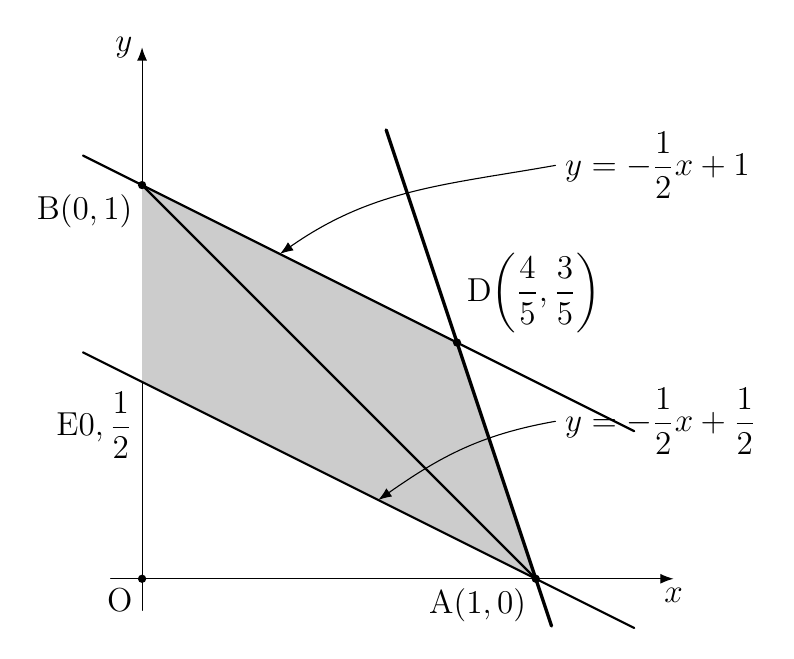
\begin{tikzpicture}[
  x=5cm,
  y=5cm,
  line cap=round,
  line join=round,
  every node/.style={font=\large}
]
  % 各点
  \coordinate (O) at (0,0);
  \coordinate (A) at (1,0);
  \coordinate (B) at (0,1);
  \coordinate (P) at (4/5,3/5);
  \coordinate (Q) at (0,1/2);

  % 座標軸
  \draw[-{Latex}] (-0.08,0)--(1.35,0)
    node[below] {$x$};
  \draw[-{Latex}] (0,-0.08)--(0,1.35)
    node[left] {$y$};

  % 斜線領域
  \fill[black!20] (Q)--(B)--(P)--(A)--cycle;

  % BとPを通る直線
  \draw[thick,domain=-0.15:1.25,samples=2]
    plot (\x,{-0.5*\x+1});

  % Aを通る平行線
  \draw[thick,domain=-0.15:1.25,samples=2]
    plot (\x,{-0.5*\x+0.5});

  % PとAを通る直線 y=-3x+3
  \draw[very thick,domain=0.62:1.04,samples=2]
    plot (\x,{-3*\x+3});

  % 点
  \foreach \X in {O,A,B,P}
    \fill (\X) circle[radius=1.5pt];

  % 点名・座標
  \node[below left] at (O) {O};
  \node[below left]      at (A) {A$(1,0)$};
  \node[below left]       at (B) {B$(0,1)$};
  \node[above right] at (P)
    {D$\left(\dfrac45,\dfrac35\right)$};

  % 直線の式
  \node[above right] at (0.05,1.08)
    {};

  \node[below left] at (0.45,0.275)
    {};
    \node[right] (eqUpper) at (1.05,1.05)
  {$y=-\dfrac12x+1$};

\draw[thin,-{Latex}]
  (eqUpper.west)
  to[out=190,in=35]
  (0.35,0.825);

% 下側の直線
\node[right] (eqLower) at (1.05,0.40)
  {$y=-\dfrac12x+\dfrac12$};

\draw[thin,-{Latex}]
  (eqLower.west)
  to[out=190,in=35]
  (0.60,0.20);
\node[below left]at(0,{1/2}){E$\p{0,\dfrac{1}{2}}$};
\draw[thick](0,1)--(1,0);
\end{tikzpicture}
\end{center}
これより,
\begin{align*}
  &\Sankaku{OAB}=\dfrac{1}{2}\\
  &\Sankaku{BAD}=\dfrac{1}{2}\det\B{\tvec<0,1>[1,-1],\tvec<0,1>[\frac{4}{5},-\frac{2}{5}]}=\dfrac{1}{5}\\
  &\Sankaku{BEA}=\dfrac12\cdot\dfrac12\times1=\dfrac14\\
  &四角形\mathrm{OADB}=\Sankaku{BAD}+\Sankaku{BEA}=\dfrac{9}{20}
\end{align*}
$\Y\Sankaku{OAB}:四角形\mathrm{OADB}=\dfrac{1}{2}:\dfrac{9}{20}=1:\dfrac{9}{10}$\\
$\Y \ans{\dfrac{9}{10}倍}$
\newpage
\noindent\ba{1$\bullet$4}\theme{ベクトルの回転と写像}\\
\kangaekata 式を観察してみると,変数を減らすことができます.（$t,u$を括れる）これを行うと,それぞれ基底ベクトルを$90\ddo$回転させたということが図形的
に読み取ることがきます.あとは,頑張って$t,u$を動かして,軌跡を求めましょう.そして,直交座標系に反感します.\\
\hokukai $C,L$をぞれぞれ変形すると,
\begin{align*}
  &C：\tvec<0,1>[x,y]=\tvec<0,1>[2t-t^2,t+2t^2]=t\tvec<0,1>[2,1]+t^2\tvec<0,1>[-1,2]\\
  &L：\tvec<0,1>[x,y]=\tvec<0,1>[2u-1,u+2]=u\tvec<0,1>[2,1]+\tvec<0,1>[-1,2]
\end{align*}
これより,$\tvec<0,1>[2,1],\tvec<0,1>[-1,2]$を基底とする$XY$斜交座標系で考えて,$t,u$を全実数で動かすと,下図を得る.
\begin{center}
  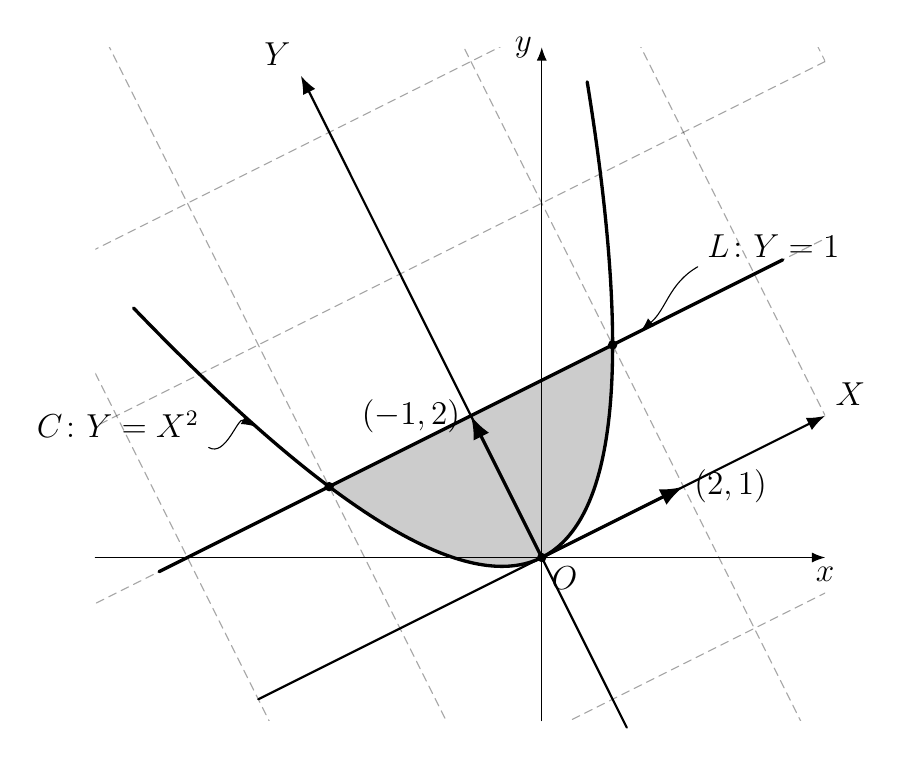
\begin{tikzpicture}[
  x=0.9cm,
  y=0.9cm,
  line cap=round,
  line join=round,
  every node/.style={font=\large}
]
  % 標準座標での主要点
  \coordinate (O)  at (0,0);
  \coordinate (E1) at (2,1);
  \coordinate (E2) at (-1,2);
  \coordinate (P1) at (-3,1); % X=-1,Y=1
  \coordinate (P2) at (1,3);  % X=1,Y=1

  % 描画範囲
  \begin{scope}
    \clip (-6.3,-2.3) rectangle (4.0,7.2);

    % 斜交座標の格子
    % (X,Y) -> (x,y)=(2X-Y,X+2Y)
    \foreach \k in {-3,-2,-1,1,2,3}{
      % Y=k
      \draw[thin,densely dashed,opacity=0.35]
        ({-10-\k},{-5+2*\k})
        --
        ({10-\k},{5+2*\k});

      % X=k
      \draw[thin,densely dashed,opacity=0.35]
        ({2*\k+5},{\k-10})
        --
        ({2*\k-5},{\k+10});
    }

    % Y=X^2 と Y=1 で囲まれる部分
    \fill[black!20]
      (P1)
      plot[
        domain=-1:1,
        samples=100,
        variable=\t
      ]
      ({2*\t-\t*\t},{\t+2*\t*\t})
      --cycle;
  \end{scope}

  % 通常の直交座標軸
  \draw[-{Latex}] (-6.3,0)--(4.0,0)
    node[below] {$x$};
  \draw[-{Latex}] (0,-2.3)--(0,7.2)
    node[left] {$y$};

  % 斜交座標のX軸・Y軸
  \draw[-{Latex},thick]
    (-4,-2)--(4,2)
    node[above right] {$X$};

  \draw[-{Latex},thick]
    (1.2,-2.4)--(-3.4,6.8)
    node[above left] {$Y$};

  % 基底ベクトル
  \draw[-{Latex},very thick]
    (O)--(E1)
    node[right] {$\left(2,1\right)$};

  \draw[-{Latex},very thick]
    (O)--(E2)
    node[left] {$\left(-1,2\right)$};

  % 曲線 C
  % (x,y)=(2t-t^2,t+2t^2)
  \draw[very thick]
    plot[
      domain=-1.6:1.6,
      samples=150,
      variable=\t
    ]
    ({2*\t-\t*\t},{\t+2*\t*\t});

  % 直線 L
  % (x,y)=(2u-1,u+2)
  \draw[very thick]
    plot[
      domain=-2.2:2.2,
      samples=2,
      variable=\u
    ]
    ({2*\u-1},{\u+2});

  % 交点と原点
  \foreach \P in {O,P1,P2}
    \fill (\P) circle[radius=1.7pt];

  \node[below right] at (O) {$O$};

  % 曲線名
  \node[below left] (curveLabel) at (-4.7,2.2)
    {$C\colon Y=X^2$};

  \draw[thin,-{Latex}]
    (curveLabel.south east)
    to[out=-30,in=150]
    (-4.05,1.85);

  % 直線名
  \node[right] (lineLabel) at (2.2,4.4)
    {$L\colon Y=1$};

  \draw[thin,-{Latex}]
    (lineLabel.south west)
    to[out=210,in=40]
    (1.4,3.2);
\end{tikzpicture}
\end{center}
これより,$XY$座標系では,
$\begin{cases}
C\colon Y=x^2\\
L\colon Y=1  
\end{cases}$なので,$CとL$の囲む面積は,
\begin{align*}
  \dint{-1}{1}\p{1-X^2}dX=\dfrac16\p{1+1}^{1+1+1}=\dfrac{4}{3}
\end{align*}
ここで,「$XY$座標での面積1」は,「$xy$座標での面積5」に相当する.$\p{\because\left|\det\B{\tvec<0,1>[2,1],\tvec<0,1>[-1,2]}\right|=5}$\\
$\Y S=\dfrac{4}{3}\times5=\ans{\dfrac{20}{3}}$
\newpage
\subsection{空間内の一次独立・符号付き長さ}
\noindent\ba{2$\bullet$1}\theme{符号付き長さ}\\
\hokukai\kakkoichib $\vec{a}\cdot\vec{b}=12$より,
\begin{align*}
  &\G{\vec{a}の\vec{b}向き符号付き長さ}=\dfrac{12}{9}=\ans{\dfrac43}\\
  &\G{\vec{b}の\vec{a}向き符号付き長さ}=\dfrac{12}{4}=\ans{3}
\end{align*}
\kakkonib$\Vec{AB}=\tvec<0,1>[1,1],\Vec{AC}=\tvec<0,1>[1,0]$なので,$\Vec{AB}\cdot\Vec{AC}=\ans{1}$\\
これより,それぞれの符号付き長さは,
\begin{align*}
  &\G{\Vec{AB}の\Vec{AC}向き符号付き長さ}=\ans{1}\\
  &\G{\Vec{AC}の\Vec{AB}向き符号付き長さ}=\ans{\dfrac{1}{\sqrt{2}}}
\end{align*}\\
\ba{2$\bullet$2}\theme{符号付き長さを目で読み取る}\\
\hokukai\kakkoichib$\ans{内積：28,符号付き長さ：7}$\\
\kakkonib$\ans{内積：-8,符号付き長さ：-2}$
\newpage
\noindent\ba{2$\bullet$3}\theme{四面体の有名問題}\\
\hokukai まず,与えられた四面体は下図のようになっている.
\begin{center}
  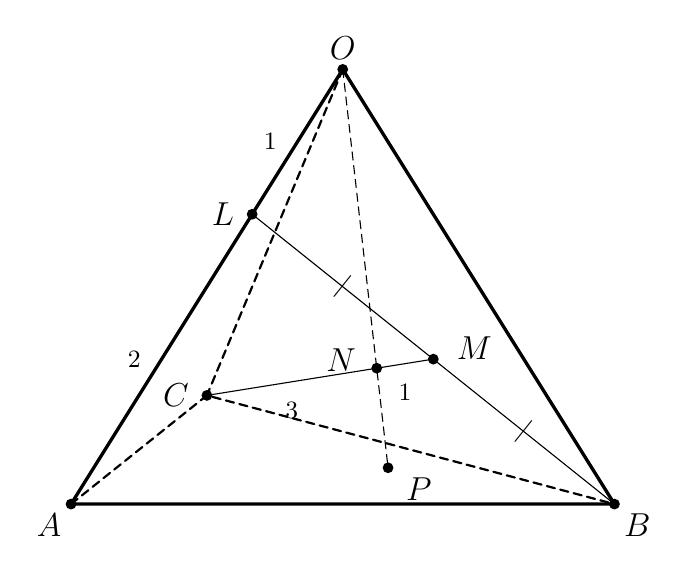
\begin{tikzpicture}[
  scale=1.15,
  line cap=round,
  line join=round,
  every node/.style={font=\large}
]
  % 四面体を平面上に射影した頂点
  \coordinate (O) at (0,4.8);
  \coordinate (A) at (-3,0);
  \coordinate (B) at (3,0);
  \coordinate (C) at (-1.5,1.2);

  % OL:LA=1:2
  \coordinate (L) at ($(O)!1/3!(A)$);

  % MはBLの中点
  \coordinate (M) at ($(B)!1/2!(L)$);

  % CN:NM=3:1
  \coordinate (N) at ($(C)!3/4!(M)$);

  % 直線ONと平面ABCとの交点
  \coordinate (P) at ($(O)!4/3!(N)$);

  % 裏側の辺
  \draw[thick,densely dashed] (O)--(C);
  \draw[thick,densely dashed] (A)--(C)--(B);

  % 四面体内部の線分
  \draw[thin] (B)--(L);
  \draw[thin] (C)--(M);
  \draw[thin,densely dashed] (O)--(P);

  % 手前側の外形
  \draw[very thick] (O)--(A)--(B)--cycle;

  % 点
  \foreach \X in {O,A,B,C,L,M,N,P}
    \fill (\X) circle[radius=1.7pt];

  % 頂点名
  \node[above]                         at (O) {$O$};
  \node[below left]                    at (A) {$A$};
  \node[below right]                   at (B) {$B$};
  \node[left,xshift=-3pt]              at (C) {$C$};

  % 内分点・交点
  \node[left,xshift=-3pt]              at (L) {$L$};
  \node[right,xshift=5pt,yshift=4pt]   at (M) {$M$};
  \node[left,xshift=-4pt,yshift=3pt]   at (N) {$N$};
  \node[below right,xshift=3pt]        at (P) {$P$};

  % MがBLの中点であることを表す印
  \path (B)--(M)
    node[midway,sloped,font=\normalsize] {$|$};
  \path (M)--(L)
    node[midway,sloped,font=\normalsize] {$|$};

  % 内分比
  \path (O)--(L)
    node[midway,left=4pt,font=\small] {$1$};
  \path (L)--(A)
    node[midway,left=4pt,font=\small] {$2$};

  \path (C)--(N)
    node[midway,below=4pt,font=\small] {$3$};
  \path (N)--(M)
    node[midway,below=4pt,font=\small] {$1$};
\end{tikzpicture}
\end{center}
\kakkoichib O,N,Pは一直線上にあるから,$\Vec{OP}=k\Vec{ON}（k\in\mathbb{R}）\cdots\cdots\maruichi$と表せる.\\
今,
\begin{align*}
  \Vec{ON}&=\Vec{OC}+\dfrac34\Vec{CM}=\vec{c}+\dfrac34\p{\Vec{OM}-\vec{c}}\\
  &=\vec{c}+\dfrac34\p{\Vec{OL}+\dfrac12\Vec{LB}-\vec{c}}\\
  &=\dfrac{1}{4}\vec{c}+\dfrac{3}{4}\B{\dfrac13\vec{a}+\dfrac12\p{\vec{b}-\dfrac13\vec{a}}}\\
  &=\dfrac18\vec{a}+\dfrac38\vec{b}+\dfrac14\vec{c}\\
  &=\dfrac{\vec{a}+3\vec{b}+2\vec{c}}{8}
\end{align*}
$\maruichi$より,$\Vec{OP}=\dfrac{k}{8}\p{\vec{a}+3\vec{b}+2\vec{c}}\cdots\cdots\maruichi^\prime$\\
一方,Pは直線ABC上にもあるので,$\Vec{OP}=\Vec{OC}+s\Vec{CA}+t\Vec{CB}（s,t：実数）$の形で表せる.\\
このとき,
\begin{align*}
  \Vec{OP}&=\vec{c}+s\p{\vec{a}-\vec{c}}+t\p{\vec{b}-\vec{c}}\\
  &=s\vec{a}+t\vec{b}+\vec{c}(1-s-t)\cdots\cdots\maruni
\end{align*}
ここで,$\vec{a},\vec{b},\vec{c}$は一次独立なので,$\maruichi^\prime$と$\maruni$の係数比較が許され,
\begin{align*}
  \begin{cases}
  \dfrac{k}{8}=s\\
  \dfrac{3k}{8}=t\\
  \dfrac{k}{4}=1-s-t
  \end{cases}\doti\begin{cases}
    s=\dfrac16\\
    t=\dfrac12\\
    k=\dfrac43
  \end{cases}
\end{align*}
$\Y\ans{\Vec{OP}=\dfrac16\vec{a}+\dfrac12\vec{b}+\dfrac13\vec{c}}$
\newpage
\noindent\kakkonib\chu 斜交座標で解答しますが,中学生的に面積比でやってもよいです.\\
Cを原点とし,$\Vec{CA},\Vec{CB}$を基底とする$XY$座標系で考えると,下図を得る.
\begin{center}
  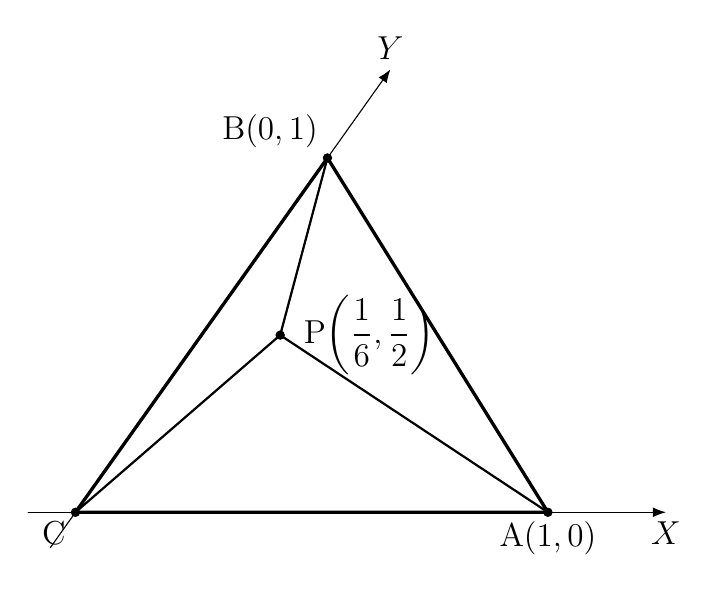
\begin{tikzpicture}[
  x={(6cm,0cm)},
  y={(3.2cm,4.5cm)},
  line cap=round,
  line join=round,
  every node/.style={font=\large}
]
  % 斜交座標
  \coordinate (C) at (0,0);
  \coordinate (A) at (1,0);
  \coordinate (B) at (0,1);
  \coordinate (P) at (1/6,1/2);

  % 斜交座標軸
  \draw[-{Latex}] (-0.10,0)--(1.25,0)
    node[below] {$X$};
  \draw[-{Latex}] (0,-0.10)--(0,1.25)
    node[above] {$Y$};

  % 三角形ABC
  \draw[very thick] (A)--(B)--(C)--cycle;

  % 内部の線分
  \draw[thick] (P)--(A);
  \draw[thick] (P)--(B);
  \draw[thick] (P)--(C);

  % 点
  \foreach \Q in {A,B,C,P}
    \fill (\Q) circle[radius=1.7pt];

  % 点名・座標
  \node[below ] at (A) {A$(1,0)$};
  \node[above left]  at (B) {B$(0,1)$};
  \node[below left]  at (C) {C};

  \node[right=5pt] at (P)
    {P$\left(\dfrac16,\dfrac12\right)$};
\end{tikzpicture}
\end{center}
直交座標系で考えても面積比は同じなので,$xy$直交座標系で考えると下図を得る.
\begin{center}
  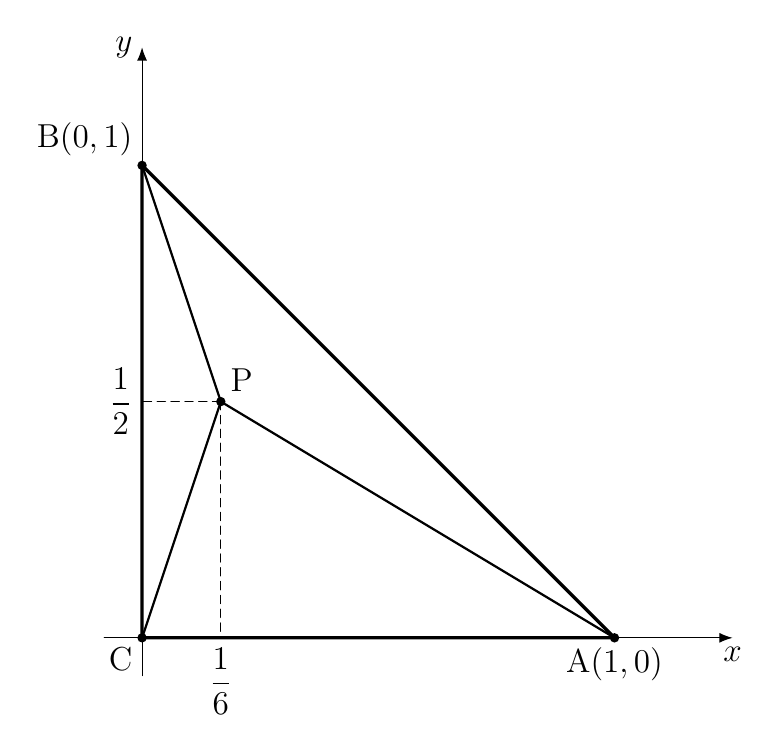
\begin{tikzpicture}[
  x=6cm,
  y=6cm,
  line cap=round,
  line join=round,
  every node/.style={font=\large}
]
  % 各点
  \coordinate (C) at (0,0);
  \coordinate (A) at (1,0);
  \coordinate (B) at (0,1);
  \coordinate (P) at (1/6,1/2);

  % 直交座標軸
  \draw[-{Latex}] (-0.08,0)--(1.25,0)
    node[below] {$x$};
  \draw[-{Latex}] (0,-0.08)--(0,1.25)
    node[left] {$y$};

  % 三角形ABC
  \draw[very thick] (A)--(B)--(C)--cycle;

  % 点Pと各頂点を結ぶ
  \draw[thick] (P)--(A);
  \draw[thick] (P)--(B);
  \draw[thick] (P)--(C);

  % Pから座標軸へ下ろした補助線
  \draw[thin,densely dashed] (P)--(1/6,0);
  \draw[thin,densely dashed] (P)--(0,1/2);

  % 点
  \foreach \Q in {A,B,C,P}
    \fill (\Q) circle[radius=1.7pt];

  % 点名・座標
  \node[below ] at (A) {A$(1,0)$};
  \node[above left]  at (B) {B$(0,1)$};
  \node[below left]  at (C) {C};
  \node[above right] at (P) {P};

  % 座標の表示
  \node[below] at (1/6,0) {$\dfrac16$};
  \node[left]  at (0,1/2) {$\dfrac12$};
\end{tikzpicture}
\end{center}
これより,面積比は,
\begin{align*}
  \Sankaku{ABP}\colon\Sankaku{BCP}\colon\Sankaku{CAP}&=\p{\dfrac{1}{2}-\dfrac{1}{4}-\dfrac{1}{12}}
  \colon\dfrac{1}{12}\colon\dfrac{1}{4}\\
  &=\dfrac{1}{6}\colon\dfrac{1}{12}\colon\dfrac{1}{4}\\
  &=\ans{2\colon1\colon3}
\end{align*}
\end{document}